\subsection{Contrat vierge }
La génération d'un contrat redoublant.es se fait en utilisant le fichier MCC. Le code créé ne doit dépendre que du fichier MCC. 
C'est-à-dire qu'il n'est pas censé être modifié pour fonctionner et être adapté au informations de l'année en cours (noms des UE, noms des EC...). 
Voici un aperçu du haut du contrat vierge :

\begin{figure}[ht]
    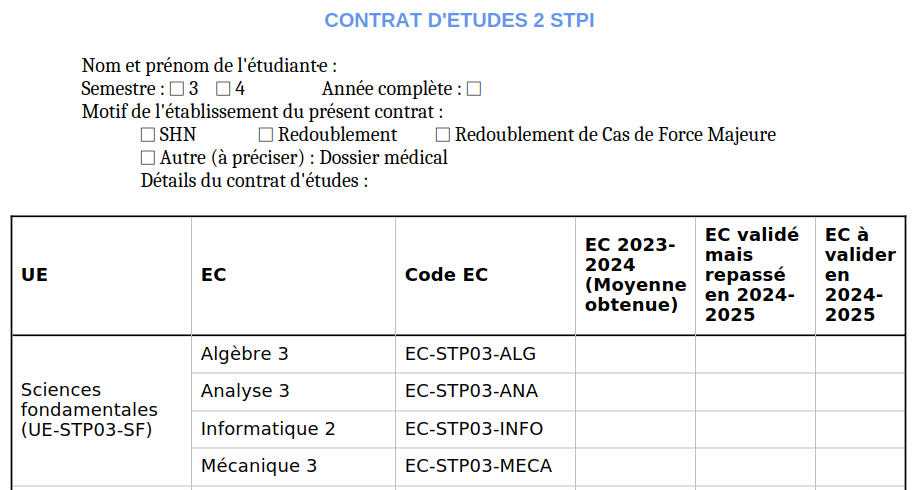
\includegraphics[width=\linewidth]{images/contrat_vierge.jpg}
    \caption{Entête du contrat vierge}
    \label{contrat_vierge}
\end{figure}

Le contrat contient aussi un espace dedié à sa signature. Celui-ci est situé à la fin du contrat.
Cette espace permet à l'étudiant.e ainsi qu'à à la personne en charge de la direction du département STPI de signer le contrat.
Il y a aussi un espace pour apposer le cachet de l'établissement.

\begin{figure}[ht]
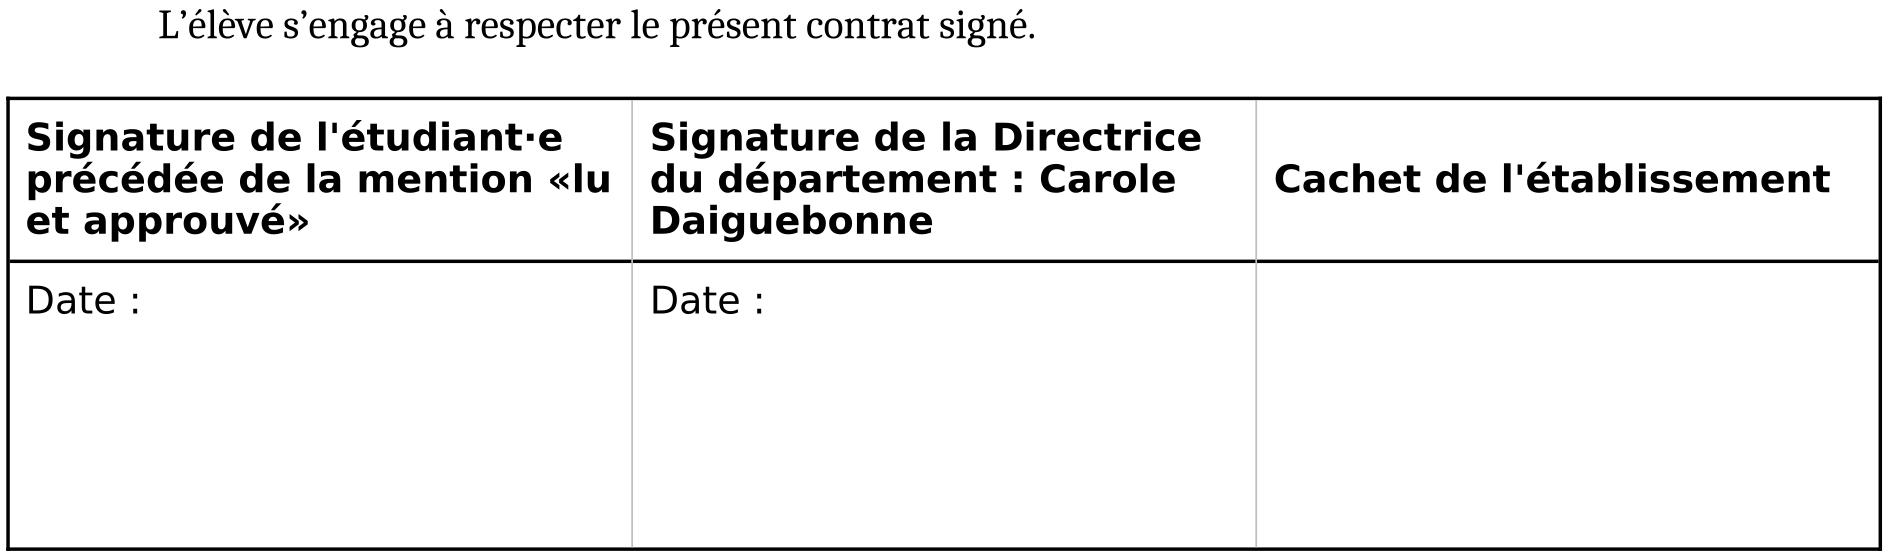
\includegraphics[width=\linewidth]{images/signature.jpg}
\caption{Espace de signature du contrat}
\label{signature}
\end{figure}


\subsection{Contrat avec notes }
Après avoir généré des notes dans le fichier jury.xlsx, nous pouvons générer des contrats pour les redoublant.es.
Cette génération ressemble à celle du contrat vierge. Il suffit de fournir le nom et le prénom d'un.e étudiant.e à la fonction de génération du contrat pour le générer.
Cette fonction appelée "generation" prend en paramètres le nom et le prénom de l'étudiant.e ainsi que le document Word qui contiendra le contrat. 
Elle permet d'ajouter automatiquement les notes de l'étudiant.e dans la colonne "EC 2024-2025 (Moyenne obtenue)". De plus, des croix sont ajoutées dans la colonne "EC à valider en 2024-2025" 
si un UE n'est pas validé et que la moyenne de l'élève à l'EC est inférieure à 10.
Les informations de validation se trouvent dans le fichier jury.xlsx.
Les nom et prénom de l'élève sont aussi ajoutés en haut du contrat à l'emplacement désigné.
Voici le contrat avec les notes de l'étudiant.e Nom1 Prenom1 issues du fichier jury de la figure ...:

  %\begin{figure}[ht]
%    \includegraphics[width=\linewidth]{contrat_notes.jpg}
%    \caption{Entête du contrat vierge}
%    \label{un-identifiant}
%\end{figure}
